\section{System Design}
\subsection{Summary Design}
\subsubsection{System Function Analysis}

Based on the information we collected from hospital management needs currently, the following functions of the management system are expected to be achieved:
\begin{enumerate}
    \item User Management Module
    \begin{enumerate}
        \item The administrator can create/modify/delete the details of other owners, including the password.
        \item Non-administrators can modify their own relevant information.

    \end{enumerate}
    \item Receptionist module
    \begin{enumerate}
        \item The reception receives appointment from patient, then they add the appointment into the system, message will be sent to doctor automatically.
        \item After doctor determines which medicine patient should take, they will send the result to reception by system, pricing and charging will be done and the patient can pick up their medicine in the warehouse.
    \end{enumerate}
    \item Warehouse keeper Module
    \begin{enumerate}
        \item The warehouse module can add, modify, delete, and query detailed drug information.
        \item Warehouse manager adds the storage information before the goods are purchased in order to make sure that warehouse always have enough.
    \end{enumerate}
\end{enumerate}

According to the detailed analysis of the above functional modules, the entire electronic management system is decomposed into a module structure diagram as Figure \ref{fig:p1}.
\begin{figure}[H]
    \centering
    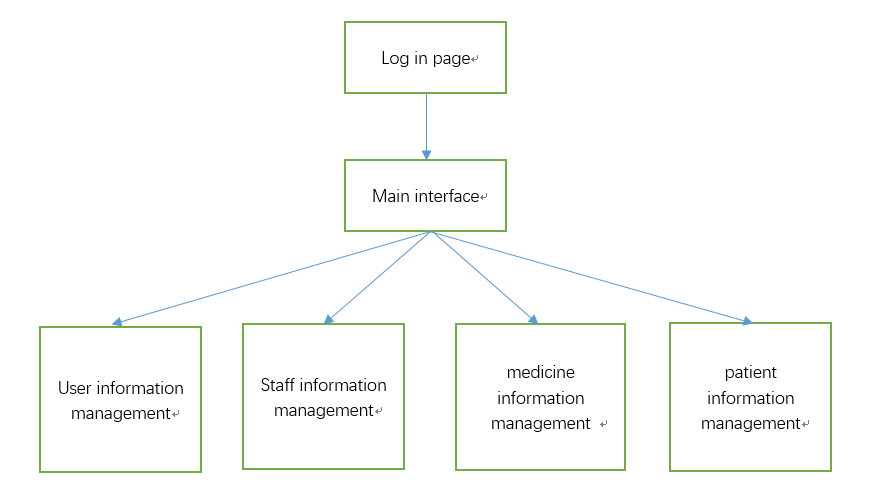
\includegraphics[width=\textwidth]{1.png}
    \caption{Module Structure Diagram }
    \label{fig:p1}
\end{figure}
\subsubsection{Detailed Design Method}

The detailed design method is divided into the most common program flowcharts, N-S box diagrams, and the IPO diagrams we will use below. Through these graphical modes, the process of our system design and development is much more clear.
\begin{enumerate}
    \item patients and doctors management model IPO
    
    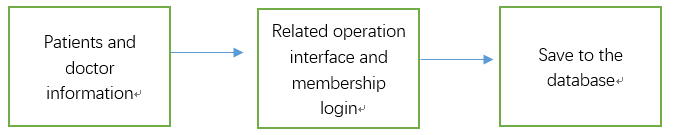
\includegraphics[width=0.9\textwidth]{2.png}
    
    \item query model IPO
    
    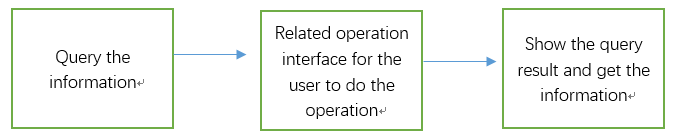
\includegraphics[width=0.9\textwidth]{3.png}

    \item charge management model IPO
    
    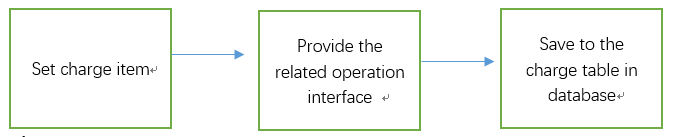
\includegraphics[width=0.9\textwidth]{4.png}

    \item user management model IPO
    
    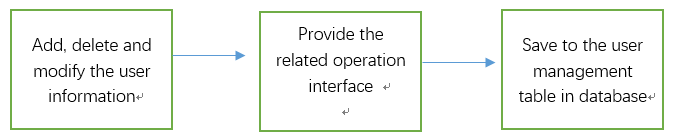
\includegraphics[width=0.9\textwidth]{5.png}

\end{enumerate}